% Created by tikzDevice version 0.8.1 on 2015-06-28 16:16:19
% !TEX encoding = UTF-8 Unicode
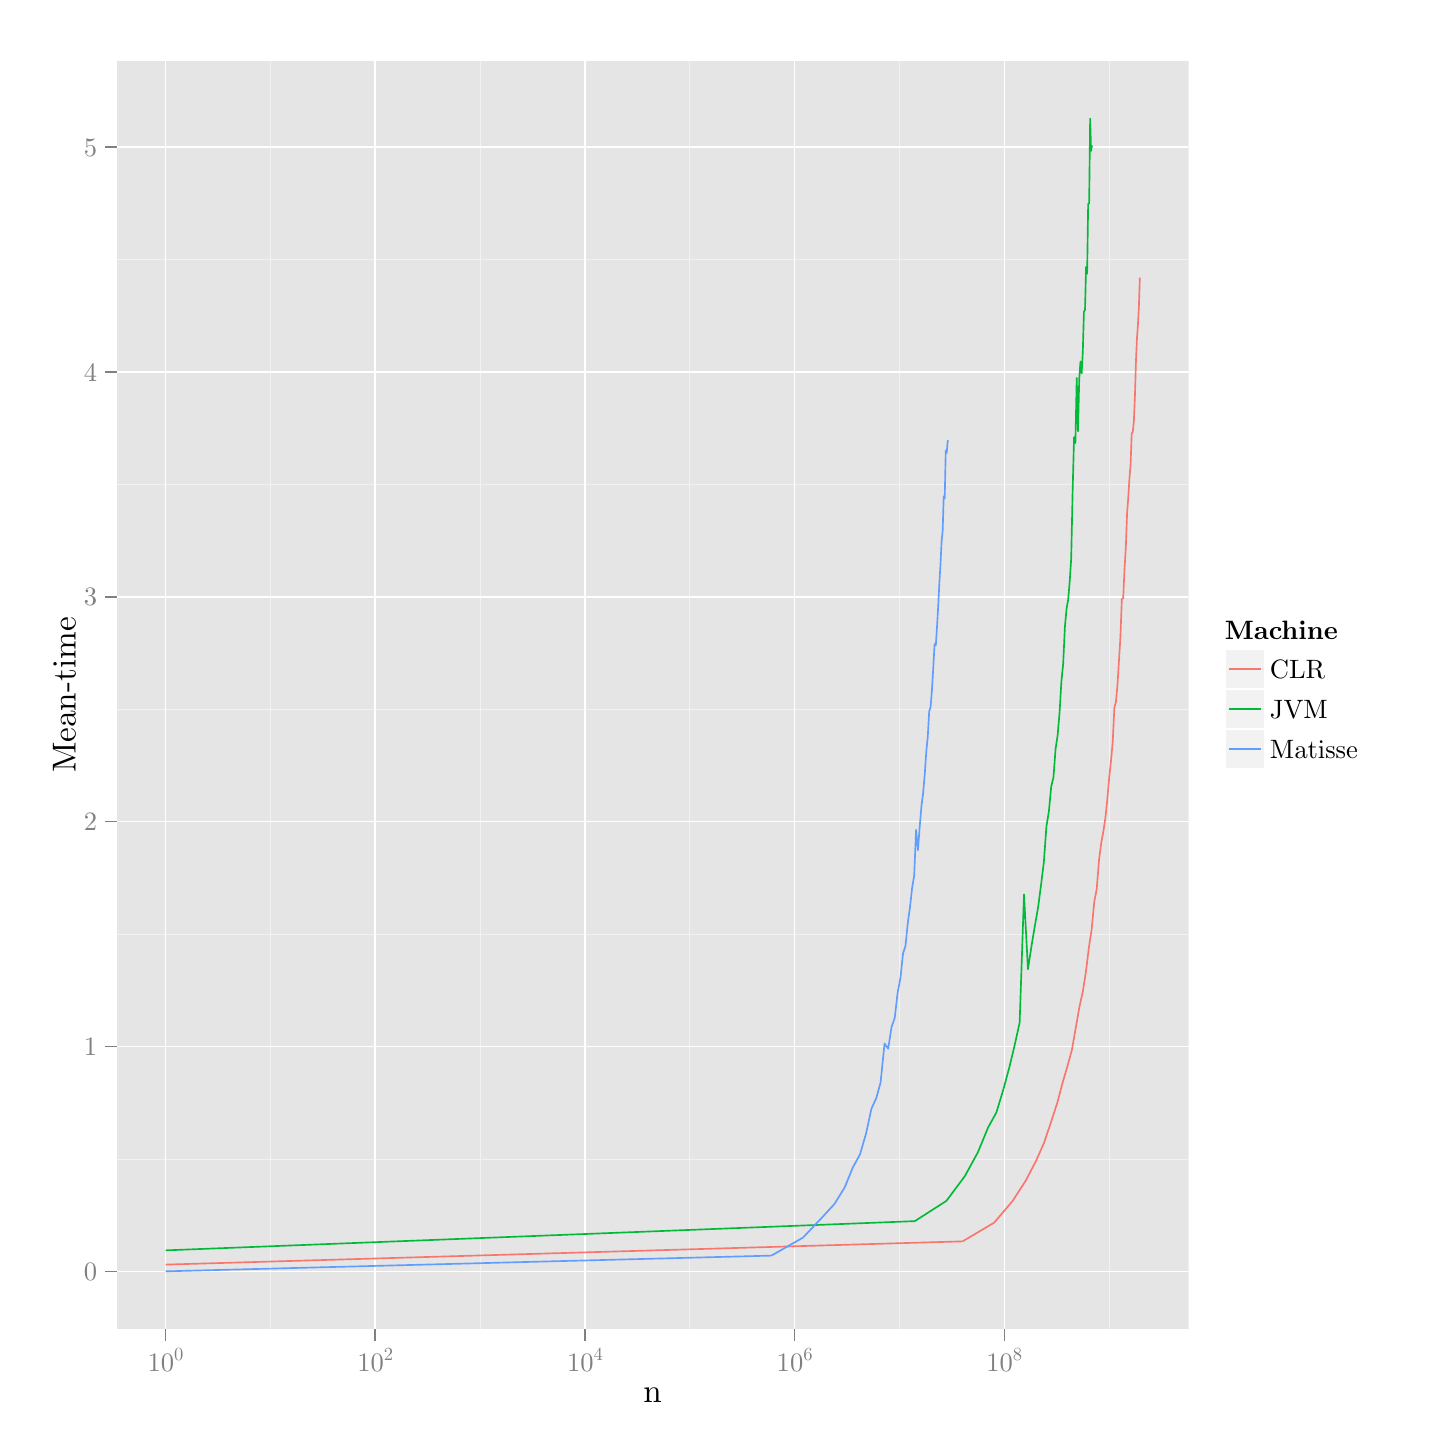
\begin{tikzpicture}[x=1pt,y=1pt]
\definecolor{fillColor}{RGB}{255,255,255}
\path[use as bounding box,fill=fillColor,fill opacity=0.00] (0,0) rectangle (505.89,505.89);
\begin{scope}
\path[clip] (  0.00,  0.00) rectangle (505.89,505.89);
\definecolor{drawColor}{RGB}{255,255,255}
\definecolor{fillColor}{RGB}{255,255,255}

\path[draw=drawColor,line width= 0.6pt,line join=round,line cap=round,fill=fillColor] (  0.00,  0.00) rectangle (505.89,505.89);
\end{scope}
\begin{scope}
\path[clip] ( 32.22, 35.66) rectangle (419.48,493.85);
\definecolor{fillColor}{gray}{0.90}

\path[fill=fillColor] ( 32.22, 35.66) rectangle (419.48,493.85);
\definecolor{drawColor}{gray}{0.95}

\path[draw=drawColor,line width= 0.3pt,line join=round] ( 32.22, 97.11) --
	(419.48, 97.11);

\path[draw=drawColor,line width= 0.3pt,line join=round] ( 32.22,178.36) --
	(419.48,178.36);

\path[draw=drawColor,line width= 0.3pt,line join=round] ( 32.22,259.61) --
	(419.48,259.61);

\path[draw=drawColor,line width= 0.3pt,line join=round] ( 32.22,340.85) --
	(419.48,340.85);

\path[draw=drawColor,line width= 0.3pt,line join=round] ( 32.22,422.10) --
	(419.48,422.10);

\path[draw=drawColor,line width= 0.3pt,line join=round] ( 87.71, 35.66) --
	( 87.71,493.85);

\path[draw=drawColor,line width= 0.3pt,line join=round] (163.48, 35.66) --
	(163.48,493.85);

\path[draw=drawColor,line width= 0.3pt,line join=round] (239.26, 35.66) --
	(239.26,493.85);

\path[draw=drawColor,line width= 0.3pt,line join=round] (315.03, 35.66) --
	(315.03,493.85);

\path[draw=drawColor,line width= 0.3pt,line join=round] (390.81, 35.66) --
	(390.81,493.85);
\definecolor{drawColor}{RGB}{255,255,255}

\path[draw=drawColor,line width= 0.6pt,line join=round] ( 32.22, 56.49) --
	(419.48, 56.49);

\path[draw=drawColor,line width= 0.6pt,line join=round] ( 32.22,137.73) --
	(419.48,137.73);

\path[draw=drawColor,line width= 0.6pt,line join=round] ( 32.22,218.98) --
	(419.48,218.98);

\path[draw=drawColor,line width= 0.6pt,line join=round] ( 32.22,300.23) --
	(419.48,300.23);

\path[draw=drawColor,line width= 0.6pt,line join=round] ( 32.22,381.48) --
	(419.48,381.48);

\path[draw=drawColor,line width= 0.6pt,line join=round] ( 32.22,462.73) --
	(419.48,462.73);

\path[draw=drawColor,line width= 0.6pt,line join=round] ( 49.82, 35.66) --
	( 49.82,493.85);

\path[draw=drawColor,line width= 0.6pt,line join=round] (125.60, 35.66) --
	(125.60,493.85);

\path[draw=drawColor,line width= 0.6pt,line join=round] (201.37, 35.66) --
	(201.37,493.85);

\path[draw=drawColor,line width= 0.6pt,line join=round] (277.14, 35.66) --
	(277.14,493.85);

\path[draw=drawColor,line width= 0.6pt,line join=round] (352.92, 35.66) --
	(352.92,493.85);
\definecolor{drawColor}{RGB}{248,118,109}

\path[draw=drawColor,line width= 0.6pt,line join=round] ( 49.82, 58.92) --
	(337.84, 67.32) --
	(349.25, 74.09) --
	(355.92, 81.94) --
	(360.65, 89.26) --
	(364.32, 96.30) --
	(367.32,103.07) --
	(369.86,110.65) --
	(372.06,117.42) --
	(373.99,124.73) --
	(375.73,130.69) --
	(377.30,136.38) --
	(378.73,144.50) --
	(380.05,152.09) --
	(381.26,157.50) --
	(382.40,164.82) --
	(383.46,173.48) --
	(384.46,179.98) --
	(385.40,190.00) --
	(386.29,194.61) --
	(387.13,205.17) --
	(387.94,211.40) --
	(388.70,215.46) --
	(389.43,220.34) --
	(390.13,227.11) --
	(390.81,234.96) --
	(391.45,240.92) --
	(392.07,247.69) --
	(392.67,260.15) --
	(393.25,262.31) --
	(393.81,268.54) --
	(394.34,277.21) --
	(394.87,285.88) --
	(395.37,299.42) --
	(395.86,299.69) --
	(396.34,310.25) --
	(396.80,317.83) --
	(397.26,330.29) --
	(397.69,335.98) --
	(398.12,343.02) --
	(398.54,348.17) --
	(398.94,359.27) --
	(399.34,359.81) --
	(399.73,363.88) --
	(400.11,373.08) --
	(400.48,385.54) --
	(400.84,393.67) --
	(401.19,398.54) --
	(401.54,405.31) --
	(401.88,415.60);
\definecolor{drawColor}{RGB}{0,186,56}

\path[draw=drawColor,line width= 0.6pt,line join=round] ( 49.82, 64.07) --
	(320.57, 74.63) --
	(331.97, 81.94) --
	(338.64, 90.88) --
	(343.38, 99.55) --
	(347.05,108.48) --
	(350.05,113.90) --
	(352.59,122.30) --
	(354.78,130.42) --
	(356.72,138.55) --
	(358.45,146.40) --
	(360.02,192.71) --
	(361.45,165.63) --
	(362.77,174.30) --
	(363.99,181.61) --
	(365.13,188.11) --
	(366.19,196.23) --
	(367.19,204.36) --
	(368.13,217.36) --
	(369.02,222.77) --
	(369.86,231.71) --
	(370.66,234.96) --
	(371.43,245.25) --
	(372.16,250.13) --
	(372.86,258.25) --
	(373.53,269.63) --
	(374.18,276.13) --
	(374.80,289.40) --
	(375.40,295.90) --
	(375.97,299.15) --
	(376.53,305.65) --
	(377.07,314.04) --
	(377.59,338.15) --
	(378.10,357.92) --
	(378.59,355.75) --
	(379.07,379.31) --
	(379.53,360.08) --
	(379.98,379.04) --
	(380.42,385.27) --
	(380.85,380.94) --
	(381.26,388.52) --
	(381.67,403.14) --
	(382.07,403.96) --
	(382.45,419.39) --
	(382.83,416.96) --
	(383.20,442.14) --
	(383.56,442.41) --
	(383.92,473.02) --
	(384.26,461.37) --
	(384.60,463.27);
\definecolor{drawColor}{RGB}{97,156,255}

\path[draw=drawColor,line width= 0.6pt,line join=round] ( 49.82, 56.49) --
	(268.74, 62.17) --
	(280.14, 68.67) --
	(286.82, 75.71) --
	(291.55, 80.86) --
	(295.22, 86.82) --
	(298.22, 94.13) --
	(300.76, 98.74) --
	(302.95,106.32) --
	(304.89,115.26) --
	(306.63,119.05) --
	(308.19,124.73) --
	(309.63,138.82) --
	(310.94,136.92) --
	(312.16,144.78) --
	(313.30,148.03) --
	(314.36,157.23) --
	(315.36,162.38) --
	(316.30,171.32) --
	(317.19,174.03) --
	(318.03,182.42) --
	(318.83,188.11) --
	(319.60,195.15) --
	(320.33,199.48) --
	(321.03,216.00) --
	(321.70,208.69) --
	(322.35,217.36) --
	(322.97,224.67) --
	(323.57,229.27) --
	(324.15,236.04) --
	(324.70,244.17) --
	(325.24,249.59) --
	(325.76,258.79) --
	(326.27,260.42) --
	(326.76,266.65) --
	(327.24,274.77) --
	(327.70,283.17) --
	(328.15,282.63) --
	(328.59,289.40) --
	(329.02,296.98) --
	(329.44,305.38) --
	(329.84,311.88) --
	(330.24,320.27) --
	(330.63,324.06) --
	(331.00,336.52) --
	(331.37,335.71) --
	(331.74,353.04) --
	(332.09,352.23) --
	(332.44,356.56) --
	(332.78,356.29);
\end{scope}
\begin{scope}
\path[clip] (  0.00,  0.00) rectangle (505.89,505.89);
\definecolor{drawColor}{gray}{0.50}

\node[text=drawColor,anchor=base east,inner sep=0pt, outer sep=0pt, scale=  0.96] at ( 25.11, 53.18) {0};

\node[text=drawColor,anchor=base east,inner sep=0pt, outer sep=0pt, scale=  0.96] at ( 25.11,134.43) {1};

\node[text=drawColor,anchor=base east,inner sep=0pt, outer sep=0pt, scale=  0.96] at ( 25.11,215.68) {2};

\node[text=drawColor,anchor=base east,inner sep=0pt, outer sep=0pt, scale=  0.96] at ( 25.11,296.92) {3};

\node[text=drawColor,anchor=base east,inner sep=0pt, outer sep=0pt, scale=  0.96] at ( 25.11,378.17) {4};

\node[text=drawColor,anchor=base east,inner sep=0pt, outer sep=0pt, scale=  0.96] at ( 25.11,459.42) {5};
\end{scope}
\begin{scope}
\path[clip] (  0.00,  0.00) rectangle (505.89,505.89);
\definecolor{drawColor}{gray}{0.50}

\path[draw=drawColor,line width= 0.6pt,line join=round] ( 27.95, 56.49) --
	( 32.22, 56.49);

\path[draw=drawColor,line width= 0.6pt,line join=round] ( 27.95,137.73) --
	( 32.22,137.73);

\path[draw=drawColor,line width= 0.6pt,line join=round] ( 27.95,218.98) --
	( 32.22,218.98);

\path[draw=drawColor,line width= 0.6pt,line join=round] ( 27.95,300.23) --
	( 32.22,300.23);

\path[draw=drawColor,line width= 0.6pt,line join=round] ( 27.95,381.48) --
	( 32.22,381.48);

\path[draw=drawColor,line width= 0.6pt,line join=round] ( 27.95,462.73) --
	( 32.22,462.73);
\end{scope}
\begin{scope}
\path[clip] (  0.00,  0.00) rectangle (505.89,505.89);
\definecolor{drawColor}{gray}{0.50}

\path[draw=drawColor,line width= 0.6pt,line join=round] ( 49.82, 31.39) --
	( 49.82, 35.66);

\path[draw=drawColor,line width= 0.6pt,line join=round] (125.60, 31.39) --
	(125.60, 35.66);

\path[draw=drawColor,line width= 0.6pt,line join=round] (201.37, 31.39) --
	(201.37, 35.66);

\path[draw=drawColor,line width= 0.6pt,line join=round] (277.14, 31.39) --
	(277.14, 35.66);

\path[draw=drawColor,line width= 0.6pt,line join=round] (352.92, 31.39) --
	(352.92, 35.66);
\end{scope}
\begin{scope}
\path[clip] (  0.00,  0.00) rectangle (505.89,505.89);
\definecolor{drawColor}{gray}{0.50}

\node[text=drawColor,anchor=base west,inner sep=0pt, outer sep=0pt, scale=  0.96] at ( 43.35, 20.31) {10};

\node[text=drawColor,anchor=base west,inner sep=0pt, outer sep=0pt, scale=  0.67] at ( 52.94, 24.24) {0};

\node[text=drawColor,anchor=base west,inner sep=0pt, outer sep=0pt, scale=  0.96] at (119.12, 20.31) {10};

\node[text=drawColor,anchor=base west,inner sep=0pt, outer sep=0pt, scale=  0.67] at (128.72, 24.24) {2};

\node[text=drawColor,anchor=base west,inner sep=0pt, outer sep=0pt, scale=  0.96] at (194.89, 20.31) {10};

\node[text=drawColor,anchor=base west,inner sep=0pt, outer sep=0pt, scale=  0.67] at (204.49, 24.24) {4};

\node[text=drawColor,anchor=base west,inner sep=0pt, outer sep=0pt, scale=  0.96] at (270.67, 20.31) {10};

\node[text=drawColor,anchor=base west,inner sep=0pt, outer sep=0pt, scale=  0.67] at (280.26, 24.24) {6};

\node[text=drawColor,anchor=base west,inner sep=0pt, outer sep=0pt, scale=  0.96] at (346.44, 20.31) {10};

\node[text=drawColor,anchor=base west,inner sep=0pt, outer sep=0pt, scale=  0.67] at (356.04, 24.24) {8};
\end{scope}
\begin{scope}
\path[clip] (  0.00,  0.00) rectangle (505.89,505.89);
\definecolor{drawColor}{RGB}{0,0,0}

\node[text=drawColor,anchor=base,inner sep=0pt, outer sep=0pt, scale=  1.20] at (225.85,  9.03) {n};
\end{scope}
\begin{scope}
\path[clip] (  0.00,  0.00) rectangle (505.89,505.89);
\definecolor{drawColor}{RGB}{0,0,0}

\node[text=drawColor,rotate= 90.00,anchor=base,inner sep=0pt, outer sep=0pt, scale=  1.20] at ( 17.30,264.75) {Mean-time};
\end{scope}
\begin{scope}
\path[clip] (  0.00,  0.00) rectangle (505.89,505.89);
\definecolor{fillColor}{RGB}{255,255,255}

\path[fill=fillColor] (428.35,233.68) rectangle (484.98,295.82);
\end{scope}
\begin{scope}
\path[clip] (  0.00,  0.00) rectangle (505.89,505.89);
\definecolor{drawColor}{RGB}{0,0,0}

\node[text=drawColor,anchor=base west,inner sep=0pt, outer sep=0pt, scale=  0.96] at (432.62,284.93) {\bfseries Machine};
\end{scope}
\begin{scope}
\path[clip] (  0.00,  0.00) rectangle (505.89,505.89);
\definecolor{drawColor}{RGB}{255,255,255}
\definecolor{fillColor}{gray}{0.95}

\path[draw=drawColor,line width= 0.6pt,line join=round,line cap=round,fill=fillColor] (432.62,266.86) rectangle (447.07,281.31);
\end{scope}
\begin{scope}
\path[clip] (  0.00,  0.00) rectangle (505.89,505.89);
\definecolor{drawColor}{RGB}{248,118,109}

\path[draw=drawColor,line width= 0.6pt,line join=round] (434.06,274.09) -- (445.62,274.09);
\end{scope}
\begin{scope}
\path[clip] (  0.00,  0.00) rectangle (505.89,505.89);
\definecolor{drawColor}{RGB}{255,255,255}
\definecolor{fillColor}{gray}{0.95}

\path[draw=drawColor,line width= 0.6pt,line join=round,line cap=round,fill=fillColor] (432.62,252.41) rectangle (447.07,266.86);
\end{scope}
\begin{scope}
\path[clip] (  0.00,  0.00) rectangle (505.89,505.89);
\definecolor{drawColor}{RGB}{0,186,56}

\path[draw=drawColor,line width= 0.6pt,line join=round] (434.06,259.63) -- (445.62,259.63);
\end{scope}
\begin{scope}
\path[clip] (  0.00,  0.00) rectangle (505.89,505.89);
\definecolor{drawColor}{RGB}{255,255,255}
\definecolor{fillColor}{gray}{0.95}

\path[draw=drawColor,line width= 0.6pt,line join=round,line cap=round,fill=fillColor] (432.62,237.95) rectangle (447.07,252.41);
\end{scope}
\begin{scope}
\path[clip] (  0.00,  0.00) rectangle (505.89,505.89);
\definecolor{drawColor}{RGB}{97,156,255}

\path[draw=drawColor,line width= 0.6pt,line join=round] (434.06,245.18) -- (445.62,245.18);
\end{scope}
\begin{scope}
\path[clip] (  0.00,  0.00) rectangle (505.89,505.89);
\definecolor{drawColor}{RGB}{0,0,0}

\node[text=drawColor,anchor=base west,inner sep=0pt, outer sep=0pt, scale=  0.96] at (448.88,270.78) {CLR};
\end{scope}
\begin{scope}
\path[clip] (  0.00,  0.00) rectangle (505.89,505.89);
\definecolor{drawColor}{RGB}{0,0,0}

\node[text=drawColor,anchor=base west,inner sep=0pt, outer sep=0pt, scale=  0.96] at (448.88,256.33) {JVM};
\end{scope}
\begin{scope}
\path[clip] (  0.00,  0.00) rectangle (505.89,505.89);
\definecolor{drawColor}{RGB}{0,0,0}

\node[text=drawColor,anchor=base west,inner sep=0pt, outer sep=0pt, scale=  0.96] at (448.88,241.87) {Matisse};
\end{scope}
\end{tikzpicture}
